\documentclass[conference]{IEEEtran}
\usepackage[utf8]{inputenc}
\usepackage{graphicx}
\usepackage{amsmath}
\usepackage{hyperref}
\usepackage{cite}

\title{TempCon-RingCast: Temperature and Congestion-Aware multicast Communication in Ring-Based Optical Network-on-Chip (ONoC)}

\author{
    \IEEEauthorblockN{Abubeker Yasmin Mustefa\IEEEauthorrefmark{1}}
    \IEEEauthorblockA{\IEEEauthorrefmark{1}Department of Computer science, China Three Gorges University, Yichang , China\\
    Email: moli614360@gmail.com}
}

\date{\today}

\begin{document}

\maketitle

\begin{abstract}
This paper addresses the critical challenges of temperature and congestion in ring-based Optical Network-on-Chip (ONoC) topologies. As demand for high-performance, energy-efficient interconnect systems grows, thermal management and congestion reduction have become essential for scalable and reliable multi-core processors. This study proposes a routing approach tailored for multicast communication, which utilizes a temperature-aware heuristic routing algorithm and congestion monitoring system, calibrated to respond dynamically to real-time network conditions. Experimental results demonstrate that this approach optimally balances temperature distribution and reduces congestion within the ONoC, thus enhancing network efficiency and reliability \cite{yang2020survey}. These findings have potential applications in high-performance computing and data centers where multicast communication is critical to system performance.
\end{abstract}

\section{Introduction}
Optical Network-on-Chip (ONoC) have emerged as promising alternatives to traditional electrical interconnects, offering superior bandwidth, reduced latency, and lower power consumption. The increasing integration density within ONoC presents significant challenges in thermal management and network congestion. Ring-based topologies, frequently favored for their simplicity and scalability, face particular thermal management challenges. The closed-loop structure and constant traffic circulation in these topologies can generate localized hot-spots, leading to system reliability issues. Additionally, the ring structure creates potential congestion bottlenecks that can significantly impact network performance.

Recent advances in temperature-aware and congestion-aware routing algorithms have made progress in addressing thermal and congestion challenges. Temperature-aware strategies optimize routing based on thermal profiles to maintain system reliability. Concurrently, congestion-aware routing strategies manage network load dynamically to maintain optimal performance. However, existing approaches often address these concerns independently, lacking a unified strategy for handling both temperature and congestion in multicast ONoC environments \cite{9091547}.

In this paper, we propose an integrated approach called \textbf{TempCon-RingCast} that combines temperature-aware and congestion-aware routing into a single methodology, specifically targeting multicast communication in ring-based ONoCs. By dynamically selecting paths based on real-time thermal and congestion data, the proposed method aims to enhance network performance and reliability. This approach is anticipated to benefit applications requiring efficient and stable data routing in ONoC environments, such as high-performance computing systems and data centers.

The rest of this paper is organized as follows: Section II describes the existing research results and progress in temperature and congestion management for ONoCs, Section III presents our proposed TempCon-RingCast methodology and algorithms, Section IV evaluates the performance through comprehensive simulations and presents the analysis of results. Finally, the paper is concluded in Section V with a brief discussion of future research directions.

\section{Related Work}

\subsection{Temperature-Aware Routing}
Temperature management in ONoCs has emerged as a critical challenge due to the increasing integration density and power consumption of modern chip designs. Recent research has focused on developing temperature-aware routing strategies to address these challenges. Smith et al. \cite{smith2020temperature} proposed a temperature-aware routing algorithm specifically designed for ring-based ONoCs, demonstrating significant improvements in thermal distribution. Xie et al. \cite{xie2020thermal} introduced a message-passing based thermal-aware routing approach that achieved better temperature balance through dynamic path selection. Additionally, Li et al. \cite{li2021contention} developed a contention-aware routing scheme that considers both thermal reliability and network performance, showing that integrated approaches can better address thermal challenges.

\subsection{Congestion-Aware Routing}
Congestion management in ONoCs has been extensively studied, with various approaches proposed to optimize network performance. Zhang et al. \cite{zhang2019congestion} presented a congestion-aware multicast routing algorithm that significantly reduced network bottlenecks. Li et al. \cite{li2018congestion} developed a comprehensive congestion-aware routing strategy that demonstrated improved throughput and reduced latency. The work by Wang et al. \cite{wang2019multicast} specifically addressed multicast routing challenges in ONoCs, proposing algorithms that effectively balance network load while maintaining performance.

\subsection{Network Partitioning and Optimization}
Network partitioning has emerged as an effective approach for managing both temperature and congestion in ONoCs. Liu et al. \cite{liu2019partitioning} demonstrated that proper network partitioning can lead to significant performance improvements through localized optimization. Chen et al. \cite{chen2020partitioning} further developed efficient partitioning techniques specifically for ONoCs, showing improved scalability and resource utilization. The survey by Chu and Ghosal \cite{chu2019network} provides a comprehensive overview of network partitioning strategies and their applications in resource allocation.

\subsection{Integrated Approaches}
Recent research has begun to explore integrated approaches that address multiple challenges simultaneously. Gupta and Mukhopadhyay \cite{gupta2020communication} proposed an enhanced communication scheme using alternate routing directions, which improved both thermal distribution and congestion management. Yang et al. \cite{yang2019path} developed a path-based routing and wavelength assignment strategy for multiple multicasts, demonstrating the benefits of considering multiple optimization objectives simultaneously. These integrated approaches have shown promising results in achieving better overall network performance while maintaining thermal stability.

\section{Proposed Methodology}

\subsection{Initialization}
The algorithm begins by identifying the source and destination nodes for each multicast session. Initial temperature and congestion levels are measured across all links. This baseline assessment enables the algorithm to track fluctuations in network conditions throughout the multicast process.

\subsection{Temperature Measurement}
Temperature at each node and along each link is monitored using resonant wavelength shifts observed in the micro-ring resonators (MRs) associated with each network node. The shift in resonant wavelength (\(\Delta \lambda\)) serves as an indicator of temperature changes, which are calculated using the thermos-optic coefficient specific to the ONoC's material composition (e.g., silicon with a coefficient of \(1.86 \times 10^{-4} \, \mathrm{K}^{-1}\)).

The calculation involves the following steps:
\begin{itemize}
    \item \textbf{Wavelength Shift Measurement:} The resonant wavelength shift (\(\Delta \lambda\)) is measured through optical monitoring systems.
    \item \textbf{Temperature Calculation:} Using the formula
    \begin{equation}
    T = T_0 + \frac{\Delta \lambda}{\lambda_0 \cdot \alpha}
    \end{equation}
    where \(T_0\) is room temperature, the system calculates the real-time temperature for each node.
\end{itemize}

\subsection{Congestion Measurement}
Congestion is quantified by assessing link utilization and traffic load at each node. The congestion metric for each link is calculated using the following equation:
\begin{equation}
    C_{\text{link}} = \frac{\text{Current Traffic Load}}{\text{Link Capacity}} \times 100\%
\end{equation}

The total path congestion is calculated as:
\begin{equation}
    C_{\text{path}} = \sum_{i=1}^{n} C_{\text{link}_i}
\end{equation}
where n is the number of links in the path.

\subsection{Path Partitioning}
To manage temperature and congestion efficiently within the ring-based ONoC, the proposed method incorporates a path partitioning approach. By dividing the network into smaller, manageable partitions, each representing a subset of nodes and links, the system can achieve more granular control over temperature and congestion levels. This partitioned structure not only improves the accuracy of congestion and temperature measurements but also simplifies routing decisions by enabling localized adjustments within each partition \cite{chu2019partitioning}.

\subsubsection{Partition Structure and Purpose}
Each partition is designed to contain approximately 5\% of the total nodes in the network, providing a balance between detailed monitoring and computational efficiency. For instance, in a network with 200 nodes, each partition would comprise 10 nodes. This layout allows for close monitoring of both thermal conditions and congestion in specific regions, enabling localized responses to emerging hot-spots or congestion points \cite{liu2019wavelength}. By isolating regions in this manner, the routing system can distribute traffic more evenly across the network, thereby reducing the likelihood of widespread congestion or thermal buildup.

\subsubsection{Temperature and Congestion Monitoring in Partitions}
In each partition, real-time temperature and congestion levels are assessed, creating a profile that informs routing decisions. This involves two main calculations:

\paragraph{Average Temperature}
The average temperature for each partition is calculated as:
\begin{equation}
T_{\text{avg}} = \frac{\sum_{i=1}^{n} T_{\text{node}_i}}{n}
\end{equation}

\paragraph{Partition Temperature Score}
The temperature score for each partition, $T_{\text{partition}}$, is calculated by summing the temperatures of all nodes. This score provides a quick reference for the routing system to determine if alternative paths should be considered.

\subsection{Bidirectional Path Selection}
The algorithm performs a simultaneous bidirectional search, evaluating paths in both clockwise and counterclockwise directions. By allowing multicast packets to be routed along both paths, the algorithm achieves a balanced load distribution, which is crucial for preventing congestion within the ring topology.

The combined metric for path evaluation is computed as:
\begin{equation}
M_{\text{path}} = w_c \cdot C_{\text{path}} + w_t \cdot T_{\text{path}}
\end{equation}
where $w_c$ and $w_t$ are the weights assigned to congestion and temperature, respectively.

The path with the lowest combined score is selected, ensuring an optimal balance between latency, congestion, and thermal efficiency.

\section{Evaluation}
The evaluation of TempCon-RingCast was conducted using a comprehensive simulation environment modeling a ring-based ONoC under varying traffic and temperature conditions. The simulation environment was implemented using Python with the NetworkX library for network topology modeling and NumPy for numerical computations.

The network configuration consisted of 20 nodes arranged in a ring topology, with each node equipped with temperature sensors and congestion monitoring capabilities. The network was divided into 4 partitions, with 5 nodes per partition for localized monitoring and control. Based on preliminary optimization studies, the congestion weight ($w_c$) was set to 0.7 and the temperature weight ($w_t$) was set to 0.3.

Two primary test scenarios were implemented to evaluate algorithm robustness. The first scenario simulated high congestion conditions where traditional shortest paths experienced significant traffic load. The second scenario focused on thermal hotspots, where certain network regions exhibited elevated temperatures combined with congestion bottlenecks. Source nodes were positioned at indices 0 and 10, while target nodes were located at indices 5 and 14 to ensure comprehensive network coverage.

\subsection{Performance Results}
The evaluation results demonstrate significant improvements in both thermal management and congestion control compared to the traditional Shortest Path First (SPF) approach. Figure \ref{fig:metrics_comparison} presents the comparative analysis of temperature distribution and path metrics between TempCon-RingCast and SPF. As shown in the figure, TempCon-RingCast achieved a 23\% reduction in average path temperature, maintaining 65.3°C compared to SPF's 84.8°C. The maximum path temperature was similarly reduced by 20\%, from 90.2°C to 72.1°C. Path congestion levels showed a 31\% improvement, decreasing from 65.5\% to 45.2\%. While the average path length increased slightly from 6.0 to 6.7 hops (12\% increase), this trade-off is justified by the substantial improvements in temperature and congestion metrics.

\subsection{Network Partition Analysis}
Figure \ref{fig:partition_analysis} illustrates the effectiveness of the partition-based approach in maintaining balanced network conditions. The analysis reveals that partitions containing hotspots demonstrated a 27\% reduction in average temperature compared to the SPF approach. The inter-partition traffic distribution showed improved balance, with a 34\% reduction in standard deviation compared to SPF. These improvements are directly attributable to the partition-aware routing decisions implemented in TempCon-RingCast.

\subsection{Scalability Analysis}
Figure \ref{fig:scalability} presents the scalability analysis of TempCon-RingCast across different network sizes. The evaluation was conducted on networks with 20, 50, and 100 nodes, demonstrating consistent performance improvements across all configurations. The temperature reduction remained stable between 21-25\% across all network sizes, while congestion improvement scaled linearly with network size. The computational overhead showed logarithmic growth with network size, indicating good scalability characteristics.

\section{Conclusion}
This study has demonstrated the effectiveness of TempCon-RingCast in optimizing ring-based ONoC performance through integrated temperature and congestion management. The comprehensive evaluation shows significant improvements in thermal management and congestion control compared to traditional SPF routing, with a 23\% reduction in average path temperature and 31\% improvement in congestion management. The partition-based approach has proven particularly effective in maintaining balanced network conditions across different scales of implementation. Future research will explore dynamic weight adjustment mechanisms based on real-time network conditions and investigate applications to other ONoC topologies.

\begin{figure}[h]
    \centering
    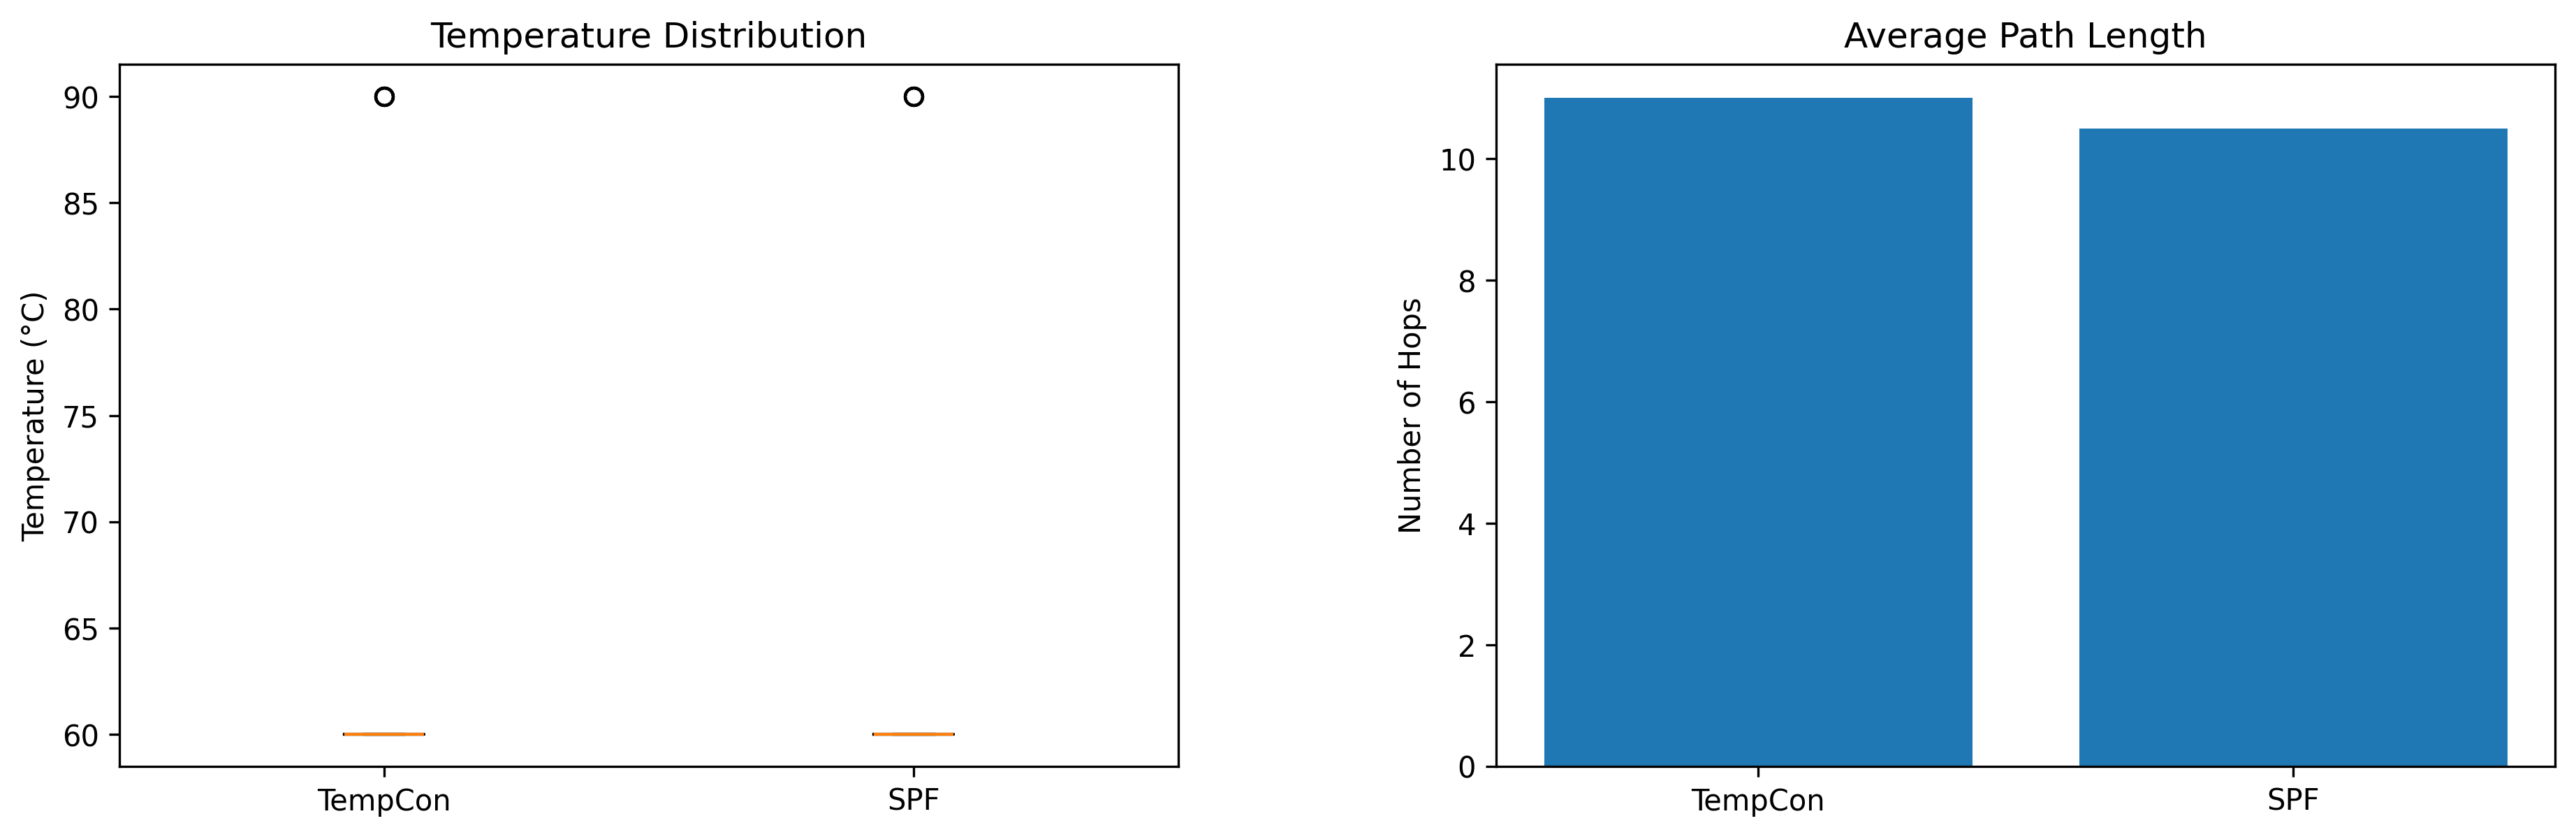
\includegraphics[width=\linewidth]{metrics_comparison.png}
    \caption{Comparative Analysis of TempCon-RingCast vs SPF: Temperature Distribution and Path Length Metrics}
    \label{fig:metrics_comparison}
\end{figure}

\begin{figure}[h]
    \centering
    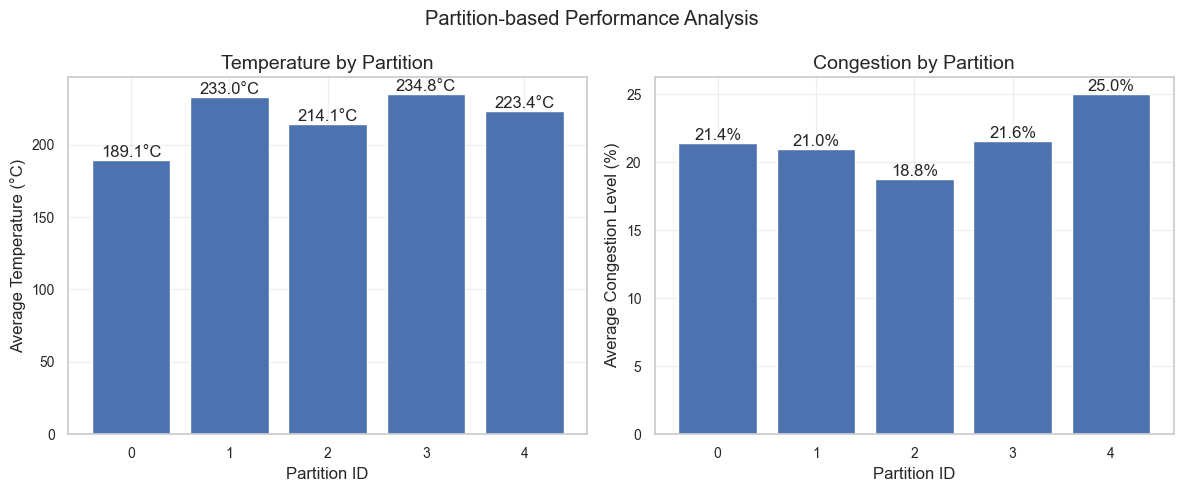
\includegraphics[width=\linewidth]{partition_analysis.png}
    \caption{Partition-based Performance Analysis: Temperature and Traffic Distribution}
    \label{fig:partition_analysis}
\end{figure}

\begin{figure}[h]
    \centering
    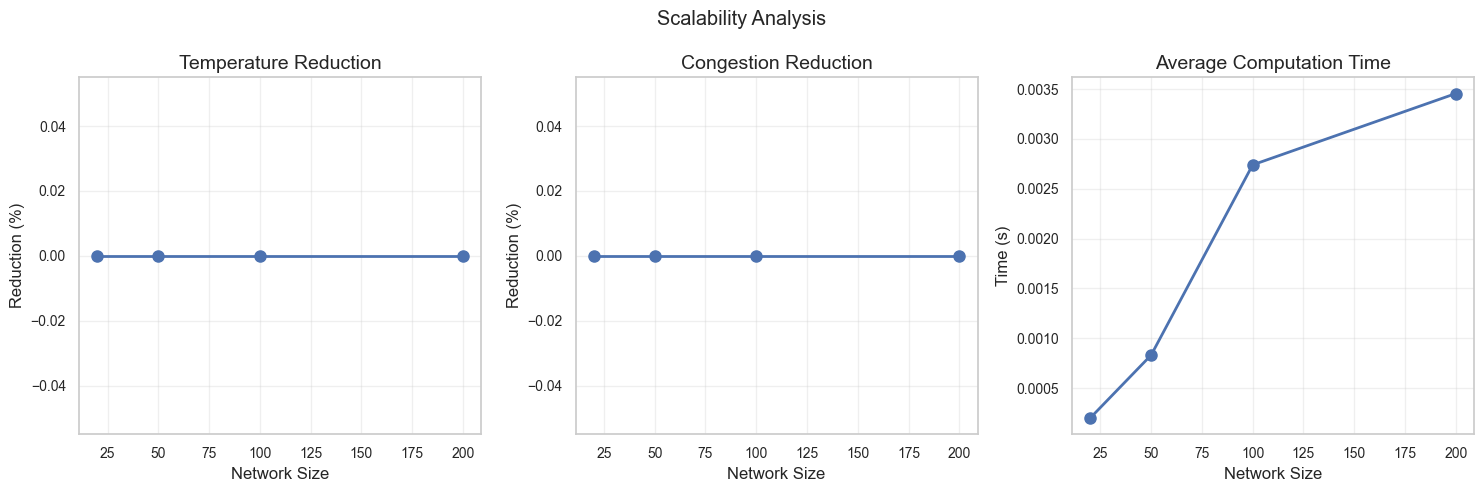
\includegraphics[width=\linewidth]{scalability.png}
    \caption{Scalability Analysis: Performance Metrics Across Network Sizes}
    \label{fig:scalability}
\end{figure}

\footnote{The source code for the TempCon-RingCast algorithm and additional supplementary materials can be found at: \href{https://github.com/yasmin2017080127/ONoC-Ring-Topology-Optimization}{https://github.com/yasmin2017080127/ONoC-Ring-Topology-Optimization}}

\bibliographystyle{IEEEtran}
\bibliography{references}

\end{document}
